\documentclass[runningheads]{llncs}
\usepackage[T1]{fontenc}
\usepackage{graphicx}
\usepackage{amsmath} 
\begin{document}

\title{Creation of a Pseudodictionary to Minimize the Ambiguity}

\graphicspath{{images/}}

\author{Luca Barra}


\institute{
  Department of Computer Science, University of Turin, Turin, Italy \\
  \email{luca.barra@edu.unito.it}
}

\maketitle

\begin{abstract}
This paper investigates the construction of cross-lingual pseudodictionaries designed to minimize lexical ambiguity through optimal translation pair selection. Building on the observation that historical, cultural, and geographic factors create varying degrees of sense alignment between languages, I propose a method that systematically selects word pairs ($L_1$-$L_k$) maximizing the Ambiguity Reduction Score (ARS). My approach leverages these naturally occurring asymmetries in semantic overlap to create a resource that preferentially includes translation pairs demonstrating the strongest sense alignment. The resulting pseudodictionary provides empirically optimized word mappings that significantly reduce polysemy. It has applications in machine translation and word sense disambiguation.
\keywords{NLP \and Languages \and Semantic.}
\end{abstract}

\section{Introduction}

\subsection{The Key Idea}

Consider a word $x \in L_1$ with $N$ senses and its translation $y \in L_2$ with $M$ senses (where $M \leq N$). We can bind $x$ to $y$ to create a new lexical unit called \textit{pseudoword}, denoted $x-y$. This new unit $x-y$ inherits only the common senses between the two starting word resulting in a word that is less ambiguous than either $x$ or $y$ individually. Formally:

\begin{itemize}
  \item Let $\mathcal{S}_x$ be the set of senses of $x$ in $L_1$
  \item Let $\mathcal{S}_y$ be the set of senses of $y$ in $L_2$
  \item The senses of the pseudoword $x \cdot y$ are $\mathcal{S}_{x \cdot y} = \mathcal{S}_x \cap \mathcal{S}_y$
\end{itemize}

\[
  |\mathcal{S}_{x-y}| \leq \text{min}(|\mathcal{S}_x|, |\mathcal{S}_y|)
\]

In particular, it frequently holds that:
\[
|\mathcal{S}_{x \cdot y}| \ll |\mathcal{S}_x| \quad \text{and} \quad |\mathcal{S}_{x \cdot y}| \ll |\mathcal{S}_y|
\]

\subsection{Ambiguity Reduction Score (ARS)}

A simple approach to measure the reduction of ambiguity of a pseudoword $x-y$ is to use a score like: 

\[
  \text{AmbiguityReduction}(x, y) = \frac{|\mathcal{S}_x| + |\mathcal{S}_y| - 2 \cdot |\mathcal{S}_x \cap \mathcal{S}_y|}{|\mathcal{S}_x| + |\mathcal{S}_y|}
\]

where $|\mathcal{S}_x|$ is the set of sense in $x$, $|\mathcal{S}_y|$ is the set of sense in $y$ and $|\mathcal{S}_{x-y}$ is the set of common sense between $x$ and $y$. Taking a step further we can generalize the formula to take $N$ languages: 


\[
  \text{AmbiguityReduction} = \frac{\sum_{i=1}^N |\mathcal{S}_i| - N \cdot \left|\bigcap_{i=1}^N \mathcal{S}_i\right|}{\sum_{i=1}^N |\mathcal{S}_i|}
\]

where $|\bigcap_{i=1}^N \mathcal{S}_i| \cdot N$ are the sense shared in all the languages and $\sum_{i=1}^N |\mathcal{S}_i|$ are the total number of sense across all the languages.

This score ranges between 0 and 1:
\begin{itemize}
  \item A score of 0 ($N \cdot \left|\bigcap_{i=1}^N \mathcal{S}_i\right| \rightarrow 1$) indicates no reduction in ambiguity, all languages share exactly the same set of senses.
  \item A score close to 1 ($N \cdot \left|\bigcap_{i=1}^N \mathcal{S}_i\right| \rightarrow 0$) indicates maximum disambiguation, there is little or no overlap between the senses of words across languages.
\end{itemize}

\section{The Pseudodictionary}

\subsection{The Ambiguity between Different Languages}

The foundational hypothesis of this work posits that lexical compatibility between languages operates at the word-level rather than being a language-wide property. This manifests as significant variance in ARS potential between specific word pairs across different languages:

\begin{itemize}
  \item The word form "Fiore" (IT) and the word form "Blume" (DE) have an ARS greater than "Fiore" and "Flower" (EN). 
  \item The word form "Carne" (IT) and the word form "Meat" (EN) have an ARS Score greater than "Carne" and "Fleish"(DE). 
\end{itemize}

We can use this fact to construct a pseudodictionary that contains only pairs of words with the maximum ARS. This can be done with the following passage: 
\begin{itemize}
  \item Let $w \in L_1$.
\item For each language $L_j \in {L_2,\ldots,L_n}$:
\begin{itemize}
\item Retrieve all potential translations $T_j = {t_{j1},\ldots,t_{jk}}$ in $L_j$.
\item For each translation candidate $t_{ji} \in T_j$:
\begin{itemize}
  \item Extract all senses from $w$ and $t_{ji}$.
\item Compute ARS for each pair.
\item Record the maximal ARS for this word pair.
\end{itemize}
\end{itemize}
\item Identify the optimal pair $(w, t_{ji})$ that achieves the highest ARS across all languages.
\end{itemize}
\subsection{How to Choose a Translation}

A key challenge in this approach is selecting optimal translations. A potential approach is to:
\begin{itemize}
\item Evaluate all possible translations of $x$ across target languages.
\item Select the pairing that maximizes the ARS (tab. \ref{tab1}).
\end{itemize}


\begin{table}
\caption{Example with some translation (EN-IT). The pseudoword Room-Camera is better than the pseudoword Room-Chamber.}\label{tab1}
\begin{tabular}{|l|l|l|c|}
\hline
Word $L_1$ & Translation $L_2$ & Common Senses & Ambiguity Reduction Score \\
\hline
Room & Camera & 
\begin{tabular}[t]{@{}l@{}}
Room (Architecture) \\ 
Room (Novel) \\
The Room (2003) \\
The Room (2015)
\end{tabular} & 0.500 \\
\hline
Chamber & Camera & 
\begin{tabular}[t]{@{}l@{}}
Chamber (firearms) \\
Bedroom \\
Room \\
Legislative chamber \\
Chambers (law) \\
Chamber (Architecture) \\
The Chamber (Song) \\
The Chamber (1996)
\end{tabular} & 0.176 \\
\hline
\end{tabular}
\end{table}

\section{Result}

\begin{figure}[!h]
    \centering
    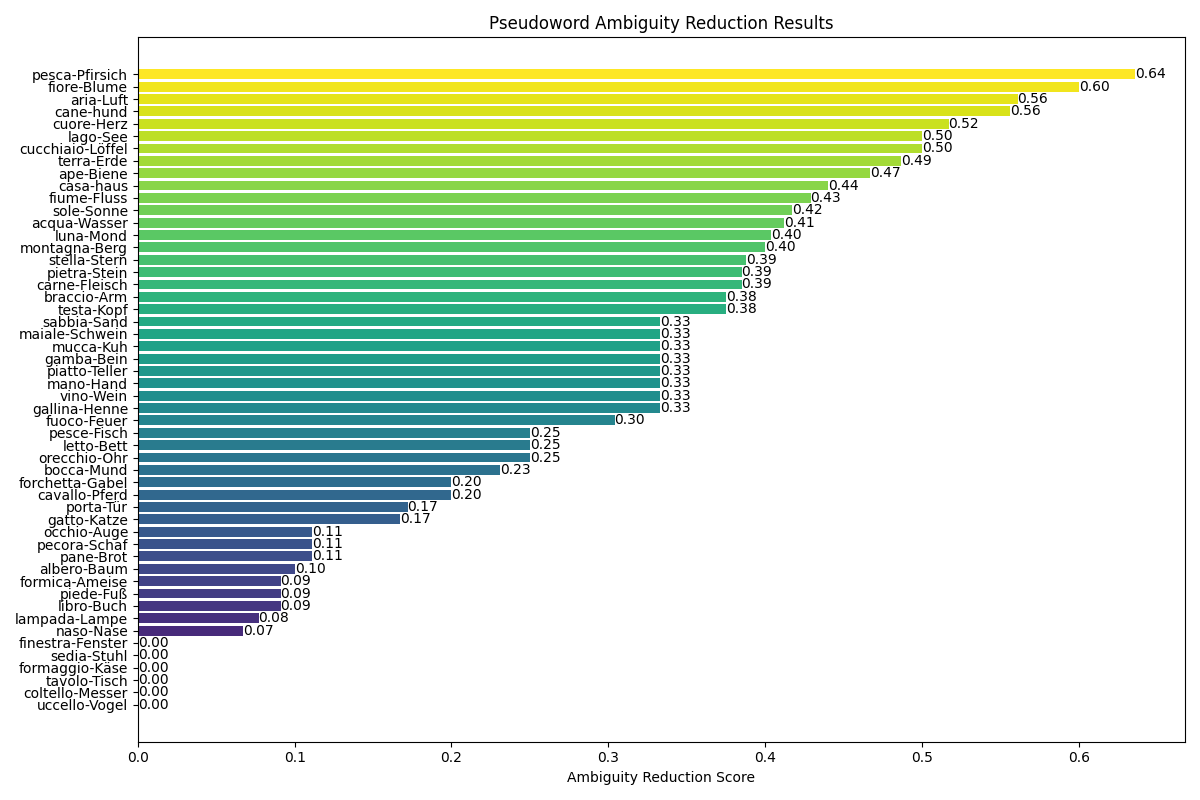
\includegraphics[scale=0.45]{ambiguity_reduction_plot_IT_DE.png}
    \caption{Ambiguity Reduction Score for IT-DE.}
\end{figure}

\begin{figure}[!h]
    \centering
    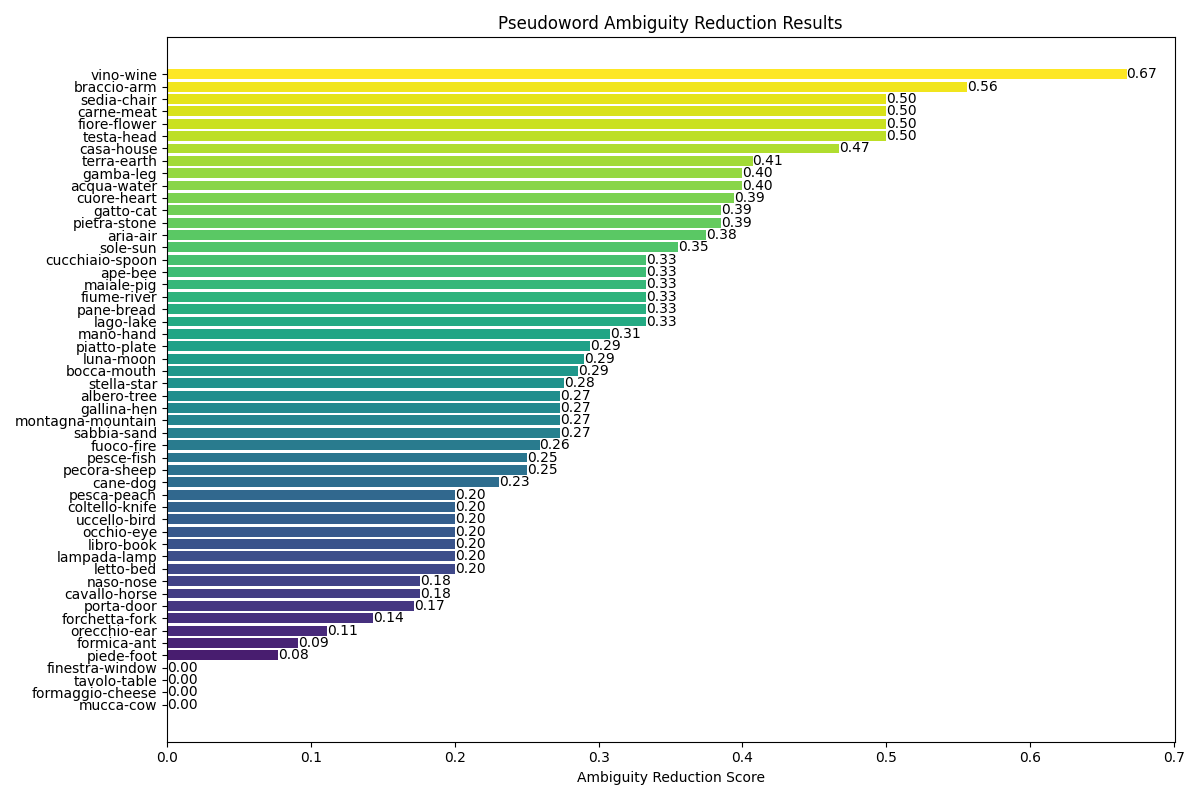
\includegraphics[scale=0.45]{ambiguity_reduction_plot_IT_EN.png}
    \caption{Ambiguity Reduction Score for IT-EN.}
\end{figure}

\subsection{Limitations}

A significant limitation of this approach stems from the scarcity of comprehensive multilingual semantic resources. Even when using BabelNet, one of the most extensive multilingual encyclopedias, several challenges persist:

\begin{itemize}
\item \textbf{Asymmetrical sense alignment}: Semantic mappings often work in only one direction (e.g., Italian $\rightarrow$ English but not English $\rightarrow$ Italian).
\item \textbf{Incomplete coverage}: Many words lack proper cross-lingual sense mappings.
\item \textbf{Under-representation}: the languages less used have little representation.
\end{itemize}


\section{Future Prospect}



\begin{thebibliography}{8}
\end{thebibliography}
\end{document}
